\documentclass[12pt,a4paper]{article}
\usepackage{lmodern}

\usepackage{amssymb,amsmath}
\usepackage{ifxetex,ifluatex}
\usepackage{fixltx2e} % provides \textsubscript
\ifnum 0\ifxetex 1\fi\ifluatex 1\fi=0 % if pdftex
  \usepackage[T1]{fontenc}
  \usepackage[utf8]{inputenc}
\else % if luatex or xelatex
  \ifxetex
    \usepackage{mathspec}
    \usepackage{xltxtra,xunicode}
  \else
    \usepackage{fontspec}
  \fi
  \defaultfontfeatures{Mapping=tex-text,Scale=MatchLowercase}
  \newcommand{\euro}{€}
\fi
% use upquote if available, for straight quotes in verbatim environments
\IfFileExists{upquote.sty}{\usepackage{upquote}}{}
% use microtype if available
\IfFileExists{microtype.sty}{%
\usepackage{microtype}
\UseMicrotypeSet[protrusion]{basicmath} % disable protrusion for tt fonts
}{}
\usepackage[lmargin = 3 cm,rmargin = 2.5cm,tmargin=2.5cm,bmargin=2.5cm]{geometry}

% Figure Placement:
\usepackage{float}
\let\origfigure\figure
\let\endorigfigure\endfigure
\renewenvironment{figure}[1][2] {
    \expandafter\origfigure\expandafter[H]
} {
    \endorigfigure
}

%% citation setup

\usepackage{csquotes}

\usepackage[backend=biber, maxbibnames = 99, style = apa]{biblatex}
\setlength\bibitemsep{1.5\itemsep}
\bibliography{references.bib}
\usepackage{color}
\usepackage{fancyvrb}
\newcommand{\VerbBar}{|}
\newcommand{\VERB}{\Verb[commandchars=\\\{\}]}
\DefineVerbatimEnvironment{Highlighting}{Verbatim}{commandchars=\\\{\}}
% Add ',fontsize=\small' for more characters per line
\usepackage{framed}
\definecolor{shadecolor}{RGB}{248,248,248}
\newenvironment{Shaded}{\begin{snugshade}}{\end{snugshade}}
\newcommand{\AlertTok}[1]{\textcolor[rgb]{0.94,0.16,0.16}{#1}}
\newcommand{\AnnotationTok}[1]{\textcolor[rgb]{0.56,0.35,0.01}{\textbf{\textit{#1}}}}
\newcommand{\AttributeTok}[1]{\textcolor[rgb]{0.77,0.63,0.00}{#1}}
\newcommand{\BaseNTok}[1]{\textcolor[rgb]{0.00,0.00,0.81}{#1}}
\newcommand{\BuiltInTok}[1]{#1}
\newcommand{\CharTok}[1]{\textcolor[rgb]{0.31,0.60,0.02}{#1}}
\newcommand{\CommentTok}[1]{\textcolor[rgb]{0.56,0.35,0.01}{\textit{#1}}}
\newcommand{\CommentVarTok}[1]{\textcolor[rgb]{0.56,0.35,0.01}{\textbf{\textit{#1}}}}
\newcommand{\ConstantTok}[1]{\textcolor[rgb]{0.00,0.00,0.00}{#1}}
\newcommand{\ControlFlowTok}[1]{\textcolor[rgb]{0.13,0.29,0.53}{\textbf{#1}}}
\newcommand{\DataTypeTok}[1]{\textcolor[rgb]{0.13,0.29,0.53}{#1}}
\newcommand{\DecValTok}[1]{\textcolor[rgb]{0.00,0.00,0.81}{#1}}
\newcommand{\DocumentationTok}[1]{\textcolor[rgb]{0.56,0.35,0.01}{\textbf{\textit{#1}}}}
\newcommand{\ErrorTok}[1]{\textcolor[rgb]{0.64,0.00,0.00}{\textbf{#1}}}
\newcommand{\ExtensionTok}[1]{#1}
\newcommand{\FloatTok}[1]{\textcolor[rgb]{0.00,0.00,0.81}{#1}}
\newcommand{\FunctionTok}[1]{\textcolor[rgb]{0.00,0.00,0.00}{#1}}
\newcommand{\ImportTok}[1]{#1}
\newcommand{\InformationTok}[1]{\textcolor[rgb]{0.56,0.35,0.01}{\textbf{\textit{#1}}}}
\newcommand{\KeywordTok}[1]{\textcolor[rgb]{0.13,0.29,0.53}{\textbf{#1}}}
\newcommand{\NormalTok}[1]{#1}
\newcommand{\OperatorTok}[1]{\textcolor[rgb]{0.81,0.36,0.00}{\textbf{#1}}}
\newcommand{\OtherTok}[1]{\textcolor[rgb]{0.56,0.35,0.01}{#1}}
\newcommand{\PreprocessorTok}[1]{\textcolor[rgb]{0.56,0.35,0.01}{\textit{#1}}}
\newcommand{\RegionMarkerTok}[1]{#1}
\newcommand{\SpecialCharTok}[1]{\textcolor[rgb]{0.00,0.00,0.00}{#1}}
\newcommand{\SpecialStringTok}[1]{\textcolor[rgb]{0.31,0.60,0.02}{#1}}
\newcommand{\StringTok}[1]{\textcolor[rgb]{0.31,0.60,0.02}{#1}}
\newcommand{\VariableTok}[1]{\textcolor[rgb]{0.00,0.00,0.00}{#1}}
\newcommand{\VerbatimStringTok}[1]{\textcolor[rgb]{0.31,0.60,0.02}{#1}}
\newcommand{\WarningTok}[1]{\textcolor[rgb]{0.56,0.35,0.01}{\textbf{\textit{#1}}}}
\usepackage{graphicx}
\makeatletter
\def\maxwidth{\ifdim\Gin@nat@width>\linewidth\linewidth\else\Gin@nat@width\fi}
\def\maxheight{\ifdim\Gin@nat@height>\textheight\textheight\else\Gin@nat@height\fi}
\makeatother
% Scale images if necessary, so that they will not overflow the page
% margins by default, and it is still possible to overwrite the defaults
% using explicit options in \includegraphics[width, height, ...]{}
\setkeys{Gin}{width=\maxwidth,height=\maxheight,keepaspectratio}
\ifxetex
  \usepackage[setpagesize=false, % page size defined by xetex
              unicode=false, % unicode breaks when used with xetex
              xetex]{hyperref}
\else
  \usepackage[unicode=true]{hyperref}
\fi
\hypersetup{breaklinks=true,
            bookmarks=true,
            pdfauthor={David Schulze, Eyayaw Teka Beze, Paffen},
            pdftitle={Whats is driving Chinese News?},
            colorlinks=true,
            citecolor=blue,
            urlcolor=blue,
            linkcolor=magenta,
            pdfborder={0 0 0}}
\urlstyle{same}  % don't use monospace font for urls
\setlength{\parindent}{0pt}
\setlength{\parskip}{6pt plus 2pt minus 1pt}
\setlength{\emergencystretch}{3em}  % prevent overfull lines
\setcounter{secnumdepth}{5}

%%% Use protect on footnotes to avoid problems with footnotes in titles
\let\rmarkdownfootnote\footnote%
\def\footnote{\protect\rmarkdownfootnote}

%%% Change title format to be more compact
\usepackage{titling}

% Create subtitle command for use in maketitle
\newcommand{\subtitle}[1]{
  \posttitle{
    \begin{center}\large#1\end{center}
    }
}

\setlength{\droptitle}{-2em}
  \title{Whats is driving Chinese News?}
  \pretitle{\vspace{\droptitle}\centering\huge}
  \posttitle{\par}
\subtitle{Linking Daily Text Data with Economic Data}
  \author{David Schulze, Eyayaw Teka Beze, Paffen}
  \preauthor{\centering\large\emph}
  \postauthor{\par}
  \predate{\centering\large\emph}
  \postdate{\par}
  \date{today}


%% linespread settings

\usepackage{setspace}

\onehalfspacing

% Language Setup

\usepackage{ifthen}
\usepackage{iflang}
\usepackage[super]{nth}
\usepackage[ngerman, english]{babel}

\begin{document}

\selectlanguage{english}


%\maketitle

\newgeometry{left=2cm,right=1cm,bottom=2cm,top=2cm}

\begin{titlepage}
  \noindent\begin{minipage}{0.6\textwidth}
	  \IfLanguageName{english}{University of Duisburg-Essen}{Universität Duisburg-Essen}\\
	  \IfLanguageName{english}{Faculty of Business Administration and Economics}{Fakultät für Wirtschaftswissensschaften}\\
	  \IfLanguageName{english}{Chair of Econometrics}{Lehrstuhl für Ökonometrie}\\
  \end{minipage}
	\begin{minipage}{0.4\textwidth}
	  \begin{flushright}
  	  \vspace{-0.5cm}
      \IfLanguageName{english}{\includegraphics*[width=5cm]{Includes/duelogo_en.png}}{\includegraphics*[width=5cm]{Includes/duelogo_de.png}}
	  \end{flushright}
	\end{minipage}
  \\
  \vspace{1.5cm}
  \begin{center}
  \huge{Whats is driving Chinese News?}\\
  \vspace{.25cm}
  \Large{Linking Daily Text Data with Economic Data}\\
  \vspace{0.5cm}
  \large{Scientifc Report}\\
  \vspace{1cm}
  \large{
  \IfLanguageName{english}{Submitted to the Faculty of \\ Business Administration and Economics \\at the \\University of Duisburg-Essen}{Vorgelegt der \\Fakultät für Wirtschaftswissenschaften der \\ Universität Duisburg-Essen}\\}
  \vspace{0.75cm}
  \large{\IfLanguageName{english}{from:}{von:}}\\
  \vspace{0.5cm}
  David Schulze, Eyayaw Teka Beze, Paffen\\
  \end{center}
  \vspace{4cm}

  \noindent\begin{minipage}[t]{0.5\textwidth}
  \IfLanguageName{english}{Matriculation Number:}{Matrikelnummer}
  \end{minipage}
  \begin{minipage}[t]{0.7\textwidth}
  \hspace{1cm}3071594, ID David, ID Eyayaw
  \end{minipage}

  \noindent\begin{minipage}[t]{0.5\textwidth}
  \IfLanguageName{english}{Study Path:}{Studienfach:}
  \end{minipage}
  \begin{minipage}[t]{0.7\textwidth}
  \hspace{1cm}Phd Programm RWI, VWL M.Sc.,
  \end{minipage}

  \noindent\begin{minipage}[t]{0.5\textwidth}
  \IfLanguageName{english}{Reviewer:}{Erstgutachter:}
  \end{minipage}
  \begin{minipage}[t]{0.7\textwidth}
  \hspace{1cm}
  \end{minipage}

  \noindent\begin{minipage}[t]{0.5\textwidth}
  \IfLanguageName{english}{Secondary Reviewer:}{Zweitgutachter}
  \end{minipage}
  \begin{minipage}[t]{0.7\textwidth}
  \hspace{1cm}
  \end{minipage}

  \noindent\begin{minipage}[t]{0.5\textwidth}
  Semester:
  \end{minipage}
  \begin{minipage}[t]{0.7\textwidth}
  \hspace{1cm}\IfLanguageName{english}{\nth{3} Semester}{3. Fachsemester}
  \end{minipage}

  \noindent\begin{minipage}[t]{0.5\textwidth}
  \IfLanguageName{english}{Graduation (est.):}{Vsl. Studienabschluss:}
  \end{minipage}
  \begin{minipage}[t]{0.7\textwidth}
  \hspace{1cm}Winter Term 2020
  \end{minipage}

  \noindent\begin{minipage}[t]{0.5\textwidth}
  \IfLanguageName{english}{Deadline:}{Abgabefrist:}
  \end{minipage}
  \begin{minipage}[t]{0.7\textwidth}
  \hspace{1cm}Apr.~7th 2020
  \end{minipage}

\end{titlepage}

% Ends the declared geometry for the titlepage
\restoregeometry


\pagenumbering{Roman} 
{
\hypersetup{linkcolor=black}
\setcounter{tocdepth}{3}
\tableofcontents
}
\newpage
\listoftables
\newpage
\listoffigures
\newpage
\pagenumbering{arabic} 
\% This command is used by pandoc when create lists and is defined in
pandoc's default latex template \providecommand{\tightlist}{%
  \setlength{\itemsep}{0pt}\setlength{\parskip}{0pt}}

\hypertarget{introduction}{%
\section{Introduction}\label{introduction}}

\hypertarget{motivation}{%
\subsection{Motivation}\label{motivation}}

Ever since it's establishment in 1948 as the Chinese Communist Party's
(CPC) officially designated publication organ, and especially since it
announced the foundation of the People's Republic by Mao Zedong on
October 1st, 1949, the People's Daily newspaper (also known as Renmin
Ribao or RMRB) has been an object of the highest interest for anyone
interested in modern China. It is safe to say that it's front page is
that of the most widely published newspapers in Chinese and it's the
most widely read. This amount of attention and it's clear designation as
voice of the CPC have made it an invaluable source for information on
China's ruling elite's communication with the masses. In times of
crisis, even tiny changes in placing, formatting or wording are chosen
and interpreted with extreme scrutiny \textcite{tan1990}. The reason for
this is on the one hand the need for some form of discussion involving
the government and the educated citizenry \textcite{kuhn2002}, but also
the sensitivity of certain topics, also called censorship.

In the past, close reading and an intimate knowledge of the Chinese
language were the only tools available to researchers interested in this
publication. Even the most well-read scholars of modern China will have
to admit that reading the paper daily and in it's entirety, even just
the front page, will be a thankless undertaking. Most articles are
official statements and collections of facts about the activites of
leaders, or plain positive messages about some aspect about the nation,
also called, by the CPC themselves, propaganda. The nuances that to
detect require years of study are difficult to check against factual
evidence, short of spending hours of reading yourself. Only rarely are
messages communicated as clearly, as back on the founding day of the
People's Republic.

This presents in our view a very urgent opportunity for automated data
mining. Unlike historic literary corpora like the works of Shakespeare
that can be analysed by generations of scholars, news is by its nature
fleeting and often needs to be analysed in a hurry and theories tested
as events unfold. Fortunately, the People's Daily offers the whole
paper's content every day for free on its homepage,
\href{http://paper.people.com.cn/rmrb/}{paper.people.com}.

To test our idea for an automated evaluation of People's Daily articles
on their own and in context of economic data, we proposed the
development of an app, that would automate the task of updating the news
corpora and economic data, as well as some descriptive and basic
analytical steps used in quantitative text analysis. To make these
results available to non-Chinese speakers, we include a simple
translation routine, that gives the most common word for word
translation, even if not the meaning of entire articles or sentences.

We stress that this will in no way substitute any qualitative reading,
knowledge of Chinese politics, expertise in Chinese language or even
text mining of the news in general. But to be able to quickly develop
and test quantitative hypotheses about Chinese news and its relation to
economic data, might be a useful tool on the way to further research and
in-depth text mining.

\hypertarget{about-the-peoples-daily-newspaper}{%
\subsection{About the People's Daily
newspaper}\label{about-the-peoples-daily-newspaper}}

For the app we focus on the first two pages, because the first is
arguably one of the most important daily publications in China, and the
second might offer interesting contrasts, because it is aimed at a
different audience, while significance diminishes rapidly with
increasing page count: The latter pages of this leading CPC publications
are actually full-page advertisements for private company's products,
among others.

The first page's layout is different every day, according to the needs
of the editors: The documentory function implies that a lot of
information is squeezed into a tight space. Articles may be reduced,
truncated or pushed to the side of the page to make room for symbolic
pictures \footnote{See for example the pictures displaying national
  remembrance of the \enquote{martyrs sacrificed in the struggle against
  Covid-19} with bowing national leaders and the lowered flag in black
  and white
  \href{http://paper.people.com.cn/rmrb/html/2020-04/05/nw.D110000renmrb_20200405_1-01.htm}{front
  page from 2020-04-05}} and voluminous leading articles. On the other
end of the spectrum are crowded front pages with up to 15 tiny articles
commemorating each meeting of a tightly packed international summit
schedule, with 15 headlines reading: \enquote{Xi Jinping meets (insert
name of foreign national head of state)} \footnote{\href{http://paper.people.com.cn/rmrb/html/2019-04/26/nbs.D110000renmrb_01.htm}{front
  page from 2020-04-26}}.

How can we ever expect to extract useful information from such a data
source? Well, for nuances in reporting to have any impact, they have to
be special or deviating in some way from an established norm. By
gathering data over hundreds of days, we hope that these patterns and
deviations will become visible. Also, comparing subsets of data such as
front and second page, reporting before and after a certain date,
commonalities will be filtered out and differences highlighted. Since
our data cover the year 2019 and the first months of the Covid-19
outbreak that was first documented officially by authorities in Wuhan,
Hubei Province China on 2020-01-05 \footnote{\enquote{Wuhan Health
  Commission report on the situation concerning a viral lung disease
  with unknown origins},
  \href{http://wjw.wuhan.gov.cn/front/web/showDetail/2020010509020}{wjw.wuhan.gov.cn}},
this constitutes an opportunity to evaluate how this major shock is
covered and news compare before and after the outbreak was acknowledged.

While text mining and natural language processing algorithms have
matured extremely in the contexts of machine learning and applications
for example in online search, the technology barrier has limited it's
adoption in the social sciences. To make basic results accessible and
reproducible, is finally a large motivation for the creation of this
app.

\hypertarget{overview}{%
\subsection{Overview}\label{overview}}

In the next sections we will introduce the general concept behind the
construction of our app, its functionality, and our general process in
coding the individual steps.

\hypertarget{construction-of-the-application}{%
\section{Construction of the
Application}\label{construction-of-the-application}}

\hypertarget{general-concept}{%
\subsection{General Concept}\label{general-concept}}

The functionality of the app has three major parts:

\begin{itemize}
\tightlist
\item
  updating databases with text and economic data
\item
  handling translation and transformation of data
\item
  outputting descriptive and analytical information
\end{itemize}

\hypertarget{shiny-user-interface}{%
\subsubsection{Shiny user interface}\label{shiny-user-interface}}

This was implement using the R package \emph{shiny}, especially
\emph{shinydashboard}, to create a layout with a tab menu on the left
hand, and a space for content on the right. Large buttons convey key
information quickly, and dynamic boxes can be filled with text, tables,
buttons, drop-down menus, and others. Especially the feature to have
tabs on top of the box to show for example several plots in one space,
was very useful.

\hypertarget{the-method}{%
\subsubsection{The method}\label{the-method}}

Formally, the functionality puts our app in the toolbox of so called
\emph{distant reading} approaches in methods of text analysis, the use
of which in social sciences in general and economics in particular is
growing.. As discussed in this
\href{http://ceur-ws.org/Vol-1786/scrivner.pdf}{workshop paper} by
\textcite{scrivner_davis2017}´, this method is not designed to
substitute or render \emph{close reading} obsolete. It actually
increases the value of such traditional methods involving a detailed
analysis of single texts, by pointing out interesting texts and features
in a growing sea of available texts. To think of an overly simple
example, compare reading a list of references to reading every single
article contained therein. The list does not give the same information,
because it abstracts from the detailed texts. But with the list, we can
find the texts we are looking for, saving time and leading to new
insights, i.e.~texts we might have missed.

The \textbf{updating} gives the user the ability to gain instant
insights in developments as they are unfolding, as soon as data are
available. The People's Daily website is updated regularly and many
other other series reachable via API are reliable sources for economic
data new enough to make this a useful feature. It is possible to extend
the app to include monthly and yearly economic data as well, but this
would be more useful, if the text data would be extended longer into the
past to match.

More precisely, our app contacts the servers of the
\href{http://paper.people.com.cn/rmrb}{Peoples Daily website}. and
economic data APIs to compare the information with our database and
check if new articles are available. If the answer is yes, it downloads
them for research purposes without intent on distribution or commercial
use and expands our database accordingly. You can find the raw
.rds-files created by scraping these articles in the folder
\enquote{/data}. Our first attempt created separate files for years and
pages, to decrease size and impact of errors. Ultimately, with
additional time, creating for example a unified SQLite database for all
objects would be computationally more efficient and lead to a
simplification of all the following code.

The \textbf{translation and transformation} aspect makes the data more
useful by offering a translation and transformed version suitable for
plotting and analysis. Having a word-for-word translation of the
newspaper data allows users to gain a limited impression of the content,
allow for quick scanning of the text by users not sufficiently
proficient in Chinese, and also allows for streamlined mining. In
particular, the free Yandex translation API used here, translates
several versions of a Chinese word to the same English correspondence.
So this n-m matching, where n\textgreater m, implies that a user who
searches using the English word will get more correct hits than for one
particular Chinese word, without necessarily losing the meaning. One of
our team members is proficient in Chinese and spot checks have confirmed
the quality of the data to be sufficient (most mistranslations concern
less common names and obscure phrases). For literary allusion and poetic
nuance, of course, the translation will necessary and always fail.

Of course all the limits of analysing language quantiatively also apply
in Chinese: Rarely is understanding a text as easy as grasping the
meaning of the individual words. For example, when searching for the
literal translation of coronavirus, recent articles will yield
surprisingly low hits. The reason is that like a lot of Chinese texts,
the news uses shorthands or less direct terms, especially for a subject
that is politically and emotionally sensitive like this one. Therefore a
better search would look for the Chinese equivalent of
\enquote{outbreak}, which in the first months of 2020 is only understood
in one way, as a reference to the pandemic.

This does not affect general inquiries, about the most frequent words
for example, in the same way. Censorship and propaganda are more obvious
on the aggregate level. It shouldn't surprise anyone to see that the
name of president Xi Jinping, the CPC and other government organs
feature highly among the most common words. This is not a mistake, but
rather revealing an important aspect of the People's Daily's reporting!

All unique Chinese article words, excluding symbols and numbers, were
translated and saved a bilingual dictionary in the folder
\enquote{/output} as a .rds-file and in comma-separated values, to allow
use in other contexts. We have gathered around 95000 unique terms over
around 15 months. For comparison, the free online dictionary
\href{https://www.mdbg.net/chinese/dictionary?page=cedict}{MDBG.net} is
based on the CC-CEDICT database which as of 2020-04-06 counts around
120000 entries, so this does not seem entirely unreasonable. In the same
folder, processed and translated copies of the articles are saved. The
process uses an NLP algorithm

\textbf{Outputting} finally is the essential part of the app: If users
can't see the result of updating and transforming the data, the app
won't be of much use. Ultimately, it would be most desireable to offer a
high degree of customization in using the app for output: Choosing
search words, specifying paramters, etc. would greatly increase its
usefulness. In the end, gathering and transforming the data proved most
time-consuming. This was to be expected, but it meant that we had to
discard our most ambitious ideas for describing, analysing and
visualising the data as well as making it interactable.

In summary, as a proof of concept, this app should show a potentially
useful application of using R with the shiny web-app, the ggplot and
other tidy packages, API connections, scraping and data mining in an
applied context.

\hypertarget{webscraping-the-peoples-daily-archive-with-rselenium-and-docker}{%
\subsection{Webscraping the People's Daily archive with Rselenium and
Docker}\label{webscraping-the-peoples-daily-archive-with-rselenium-and-docker}}

The platform CrossAsia.org is a service provided by the Staatsbibliothek
zu Berlin and funded by the DFG. It collects and offers access to data
for many kinds of Asia-related research. Through CrossAsia we have
access to a database of issues of the People's Daily starting from 1946.
The oldest edition is dated on May 15, 1946. The People's Daily website
on the other hand offers issues since the beginning of 2019 and is
offered directly to everyone on the internet.

To combine the long archive and the easy access to the new issues, we
had the idea to develop a webscraper that updates using the People's
Daily website and adds the articles to our database based on the archive
via CrossAsia.org.

Since this archive is only accessable with an account and a memebership,
for the scraping of the archive, a login for the scraping process is
necessary. The best solution to send the login credentials, browse
through the archive, and scrape the content, we came up with is an
Firefox image in Docker accessed by the RSelenium package.

Docker is a batch of so called platforms as a service (PaaS), which is a
type of cloud computing service to manage and run application without
any kind of infrastructure. For our purpose we used Docker to build a
browser in a virtual machine and then connect these with R using the
RSelenium package. For a detailed installation guideline we recommend to
have a look at
\url{https://docs.ropensci.org/RSelenium/articles/docker.html}. To
interact with the virtual browser image in R, RSelenium uses a class
called RSelenium::remoteDriver, which features several functions such as
\emph{remDr\$navigate(\enquote{url})} to browse to a specific website or
more specific ones like \emph{remDr\$screenshot()} to display or save
and screenshot of the actual webpage, or
\emph{remDr\$sendKeysToElement()} which allows the user to send specific
keys like \enquote{Enter} to the browser.

Before we can start to scrape the articles we need to start the Docker
image as explained in the guideline. Then the first thin the scraper
function \emph{ca\_scaper()} function calls is \emph{ca\_login()}. The
latter connects the remoteDriver with Docker. When this is done it
navigates to the login page of CrossAsia.org and hands over our account
credentials.

The article overview of each issue is uniformly displayed by the date
that the issue page is reached.

In this case, 19460515 for the date and 1 for page 1. The link structure
of the archive differs significantly from that of the free archive.
Besides a personal session token, in this case \enquote{s894ib9c043f},
the link structure differs by the access points to the archive. In
addition to CrossAsia.org, the Staatsbibliothek zu Berlin should be
mentioned here in particular. This can be found in the suffix
\enquote{.erf.sbb.spk-berlin.de}. The article overview of each issue is
uniformly accessible via the date and page number. LINK
\url{http://data.people.com.cn.s894ib9c043f.erf.sbb.spk-berlin.de/rmrb/19460515/1/}
In this case, 19460515 for the date and 1 for page 1. 32-character ID is
used for article archiving. LINK :
\url{http://data.people.com.cn.s894ib9c043f.erf.sbb.spk-berlin.de/rmrb/19460515/1/cae1d1ef94a74c8e99ad43189652fb40}
shows the oldest article of the archive. Since the ID does not seem to
follow a fixed pattern, it must be obtained from the article overview
for the scraping process. A list of all article IDs can be retrieved on
each overview page by using the HTML node \enquote{li h3 a} and the
attribute \enquote{href}. Now links can be generated from the date
format and the IDs to call up the individual articles. To fullfill this
task the scraper calls the function ca\_date\_urls. The so created url
list is then passed to \emph{ca\_content()}.

Afterwards the scraper maps over this list while calling the
\emph{ca\_content()}-function. Almost all important information such as
author, title, subtitle and article content can be retrieved via the
html node \enquote{\#detail\_pop\_content} and the underlying nodes
\enquote{.title}, \enquote{.subtitle}, \enquote{.author}, and
\enquote{p}. After scraping the information all content is saved in a
tibble.

\hypertarget{page-protection}{%
\subsubsection{Page protection}\label{page-protection}}

Since CrossAsia.org is paying the provider of the archive a fee for the
content they give acces to, both they and the provider are oriented
towards protecting the archive data from illegal downloads. Although the
use for preview purposes is allowed, the user cannot always be
distinguished from a \enquote{data pirate}, i.e.~offering the articles
on the Internet after downloading them. In addition, the provider wants
to keep his server load as low as possible in order to grant as many
users as possible quick access to the archive at the same time. If
several users now send automated requests to the archive, this can
affect the speed of the servers. By randomly generating sleep times in
the code, the scraping behavior can be adapted to the usage behavior of
a human being. CrossAsia.org asks the user to solve a simple captcha
after a certain number of article calls. To solve these problems, our
webscraper first checks for a location in the HTML code that is present
on both the article page and the captcha page. If the site structure
equals the one of a saved version of the captcha site the function
\emph{ca\_captcha()} is called.

First, a screenshot of the page is saved by the remoteDriver and cropped
in a way that only the captcha image is left. The page
\url{https://2captcha.com} LINK offers the possibility to solve captchas
automatically for a small fee of less than 1\$ per 1000 captchas. For
this purpose, the user is provided with an API key, which can be used to
transmit the image information as a POST request with
multipart-encoding. Afterwards, the user is assigned a ticket-ID, with
which he can retrieve the solved captcha code as a string after about
5-10 seconds of waiting time. Since the operator may sometimes
experience increased solving times, we check the content of the string.
A waiting time of 5 seconds is added if the captcha has not been solved
yet and an attempt to grab the code follows the additional waiting time.
The captcha-code is now sent to the to the corresponding form of
CrossAsia.com and will be forwarded automatically. After entering the
captcha code, we check again if the forwarding was successful or if the
entered captcha code was invalid and therefore another captcha must be
solved. Even solving these captures codes and extensive waiting time of
about 10 minutes after each page, we expierenced that the archive
operator gives a time-out error to users additionally, if they try to
look at too many articles in a given time. The time-out length and the
length until a timeout is called differs from 30 minutes to a few hours.
We tried to check for this site behavior but were not completly
succesfull in providing a function to check for the time-out and wait
until it disappears.

\hypertarget{output}{%
\subsubsection{Output}\label{output}}

In the end the intense timeout periods lead us to the decision that the
webscraping of the archive is possible but extremely time consuming. The
code will be able to scrape the content as described, but for the
purpose of the app we decided to not integrate the archive content so
far.

\hypertarget{translation-from-chinese}{%
\subsection{Translation from Chinese}\label{translation-from-chinese}}

To make the app basically usable for non-Chinese speakers, a translation
feature was introduced. Because Chinese has no spaces, we needed to use
a NLP algorithm, so that in the article texts, spaces could be placed
between words to separate them. Unique words were added to a Chinese
dictionary. Each word was in turn passed on to the translation API from
Yandex. This yields in most cases a reliable one-word translation.
Alternative translations were beyond the scope of this app, and for in
depth analysis, a knowledge of Chinese or at least use of more
translation tools is necessary. This dictionary is exported in .rds and
.csv files for further use. The articles are then translated word for
word. This will speed up using the app for text mining with English
words, even if it does not give a useful translation of the complete
texts.

\hypertarget{some-additional-remarks}{%
\subsubsection{Some additional remarks:}\label{some-additional-remarks}}

To reduce use of the Yandex translation API (which has limited free
bandwith) in each update, only new words are translated and added. This
allowed an approximation of the range of unique words used. For
illustration: Translating all the unique words (words includes here
names, idioms, technological terms, etc.) yielded at least 50150 unique
words for the first pages of all of 2019. The second pages of 2019 added
16393 new words. For the first three months, we found still 3228 new
words for page 1 and 2350 new words for page 2. Even when allowing for
misclassification by the NLP algorithm (sometimes words might be
recorded as separate and again as a compound), this suggests that the
news needs plenty of new words to adapt to current developments,
e.g.~\enquote{Covid-19}.

Another aspect of the dictionary: While all Chinese words are unique,
the English translation yielded around 25000 duplicated entries. This
means that users searching for example for \enquote{satellite} will find
hits for \enquote{Wei Xing}, \enquote{Ke Weixing} and \enquote{Renzao
Wei Xing}, which all carry that meaning, improving the accuracy of text
mining.

\hypertarget{word-frequency-time-series-and-economic-data}{%
\subsection{Word frequency time series and economic
data}\label{word-frequency-time-series-and-economic-data}}

In order to gain an impression of the impact the frequency of a single
word can have on the economy, we created the function
\emph{ts\_word\_frequency()} to generate time series and visualize the
results. The user first specifies whether he wants to search the
articles on page 1 or page 2 (page\_num) for a specific word
(eng\_word). In addition, the user can specify a time period in which
the analysis is to be performed using start\_date and end\_date. In the
parameter econ\_data he also determines whether he wants to compare the
word frequency of eng\_word with the NASDAQ\_CNY or dollar\_yuan\_exch,
which have already been explained in the section on economic data. We
have integrated a function to download them from different sources and
then adjust and, if necessary, normalize them according to the user's
input time parameters. Furthermore there is the possibility to extend
the frequency of time series from monthly to daily. It is also possible
to extend the frequency of time series from monthly to daily.

In the next step we load all articles of page 1 or 2 according to the
number of pages requested by the user and tokenize them. A token can be
described as a meaningful word, which is worth considering in the
context of a later word frequency analysis. The function which performs
this task is called \emph{tidy\_text()}. Now we have a database which
can be filtered by the user's chosen word eng\_word, and the time
period. Afterwards the values of the economic data are passed over the
filtered database and the two time series are plotted. This plot is now
transferred to the app and displayed to the user.

\hypertarget{exploratory-statistics-visualisation-and-text-mining}{%
\subsection{Exploratory statistics, visualisation, and text
mining}\label{exploratory-statistics-visualisation-and-text-mining}}

The goal for this project was to show that it is possible to create an
interactive app with live data updates, analysis and output. While this
is just an illustration to prove the concept, there are of course
limitless possibilites to extend the dataset with more economic and text
data. And all manner of econometric, natural language processing,
machine learning or corpus linguistig tools could be implemented.

In the app as it is now, we managed to implement the simplest
descriptive statistics: - An overview of the dataset that indicates time
and number of articles for page 1 and 2 respectively. - Plots of the
frequency of articles per day. - The difference between the local data
and the newest article online, and - plots of the frequency of certain
keywords per day standardized around the starting date, in comparison to
a NASDAQ index of Chinese industrial companies, also standardized the
same way.

These serve to give the user an overview and a little more understand of
the data. The article frequency per day plots show, for example, that
there are systematic differences between the first and second pages. For
both 2019 and 2020, the first page has several outliers with over 10
articles per page, while the second page has no more than 9 articles per
page. This is mostly due to the coverage over important events which are
covered in many small articles on the front page, e.g Xi Jinping's
meetings with world leaders at international summits.

But especially the time series shows the advantage of quantitative text
analysis: Now we can see for example the frequency of \enquote{Crown},
the literal translation of Corona, or equivalently the term
\enquote{outbreak}, increasing dramatically around February as expected,
coinciding with a drop in the industrial index.

Another interesting result is the frequency of \enquote{development}, a
staple of positive economic reporting and policy reports. While always
present, especially during upturns in the index, starting in February
2020 it get's remarkably displaced, most likely by reporting on the
pandemic.

Lastly this quick and large scale analysis can lead to surprising
results that warrant furher investigation: The term
\enquote{inspection}, usually associated with political control and
anti-corruption activities, has two extreme modes in the data, one
during the outbreak and one last spring. This could be related to the
spring festival, which is around February every year, or have some other
reason. The results show that this approach has potential to be a highly
useful tool for empirically testing hypothesis and developing new ones.

\begin{Shaded}
\begin{Highlighting}[]
\NormalTok{knitr}\OperatorTok{::}\KeywordTok{include_graphics}\NormalTok{(}
  \KeywordTok{c}\NormalTok{(}
\NormalTok{    here}\OperatorTok{::}\KeywordTok{here}\NormalTok{(}\StringTok{"ts_plots/outbreak.png"}\NormalTok{),}
\NormalTok{    here}\OperatorTok{::}\KeywordTok{here}\NormalTok{(}\StringTok{"ts_plots/development.png"}\NormalTok{),}
\NormalTok{    here}\OperatorTok{::}\KeywordTok{here}\NormalTok{(}\StringTok{"ts_plots/inspection.png"}\NormalTok{)}
\NormalTok{  ),}
  \DataTypeTok{dpi =} \OtherTok{NA}
\NormalTok{)}
\end{Highlighting}
\end{Shaded}

\begin{figure}

{\centering 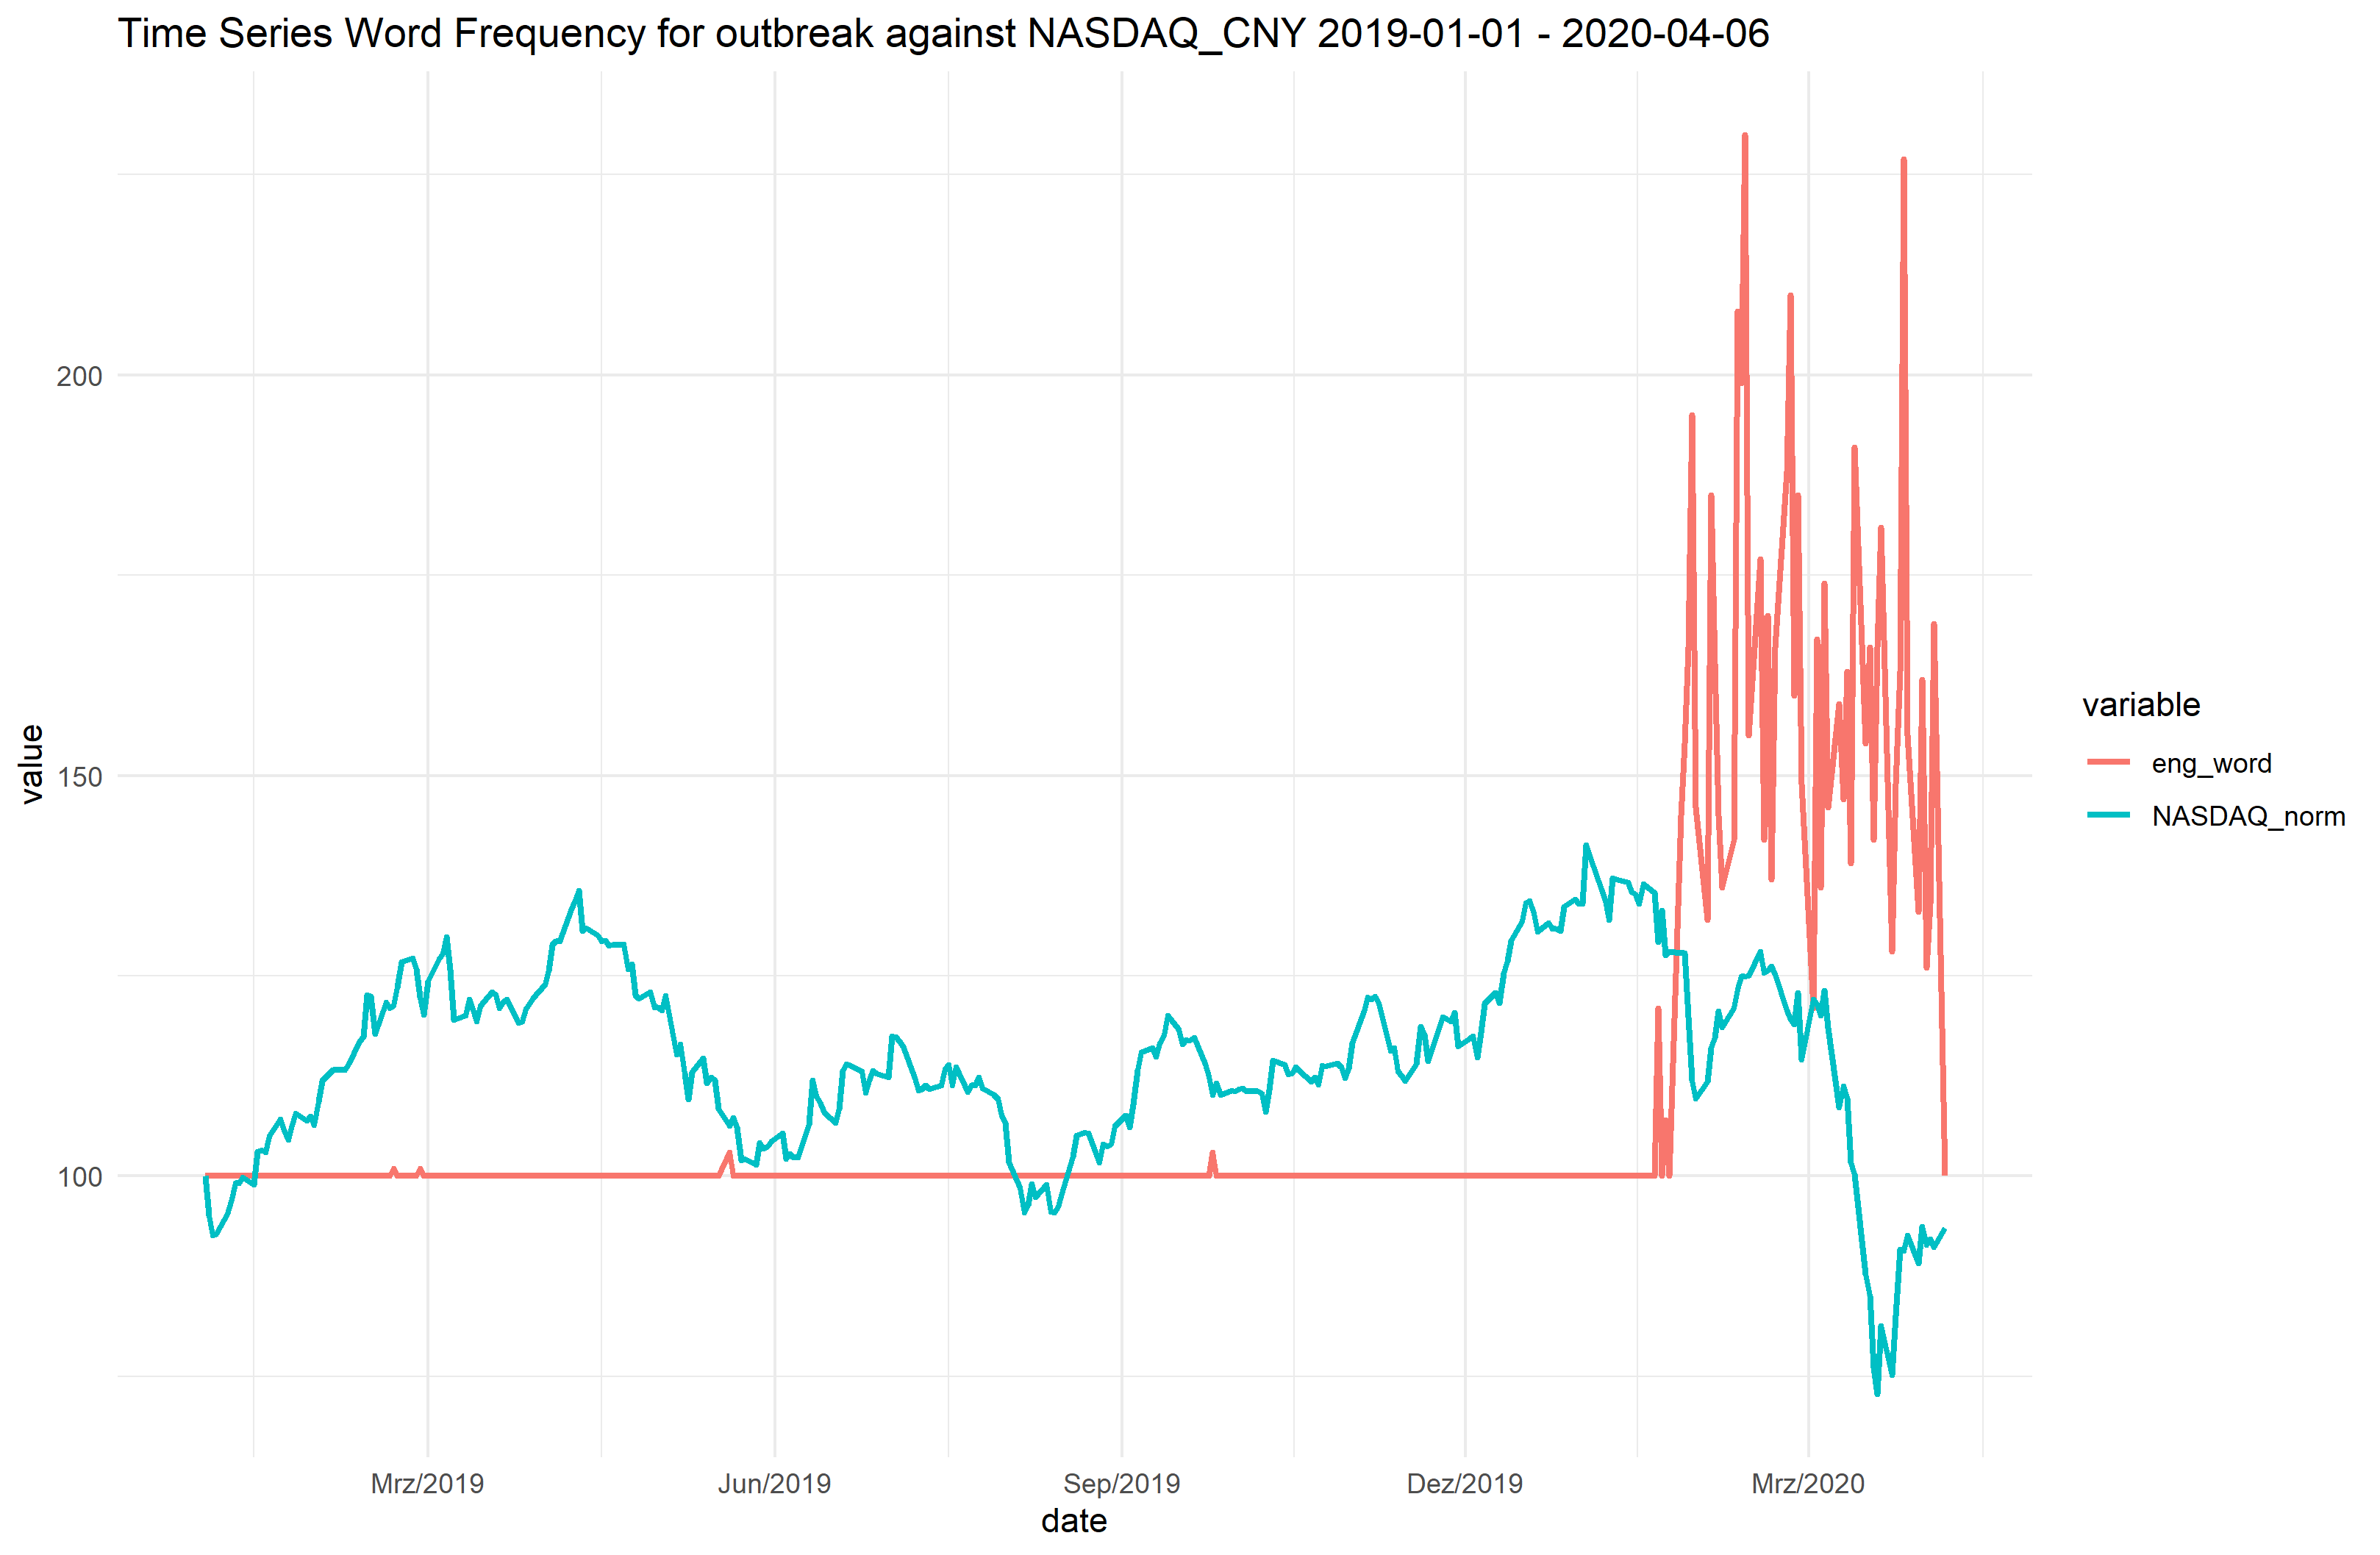
\includegraphics[width=0.49\linewidth,height=0.2\textheight]{C:/Users/David/Seafile/Meine Bibliothek/Kurse/adv-r/Advanced_R_Project/ts_plots/outbreak} 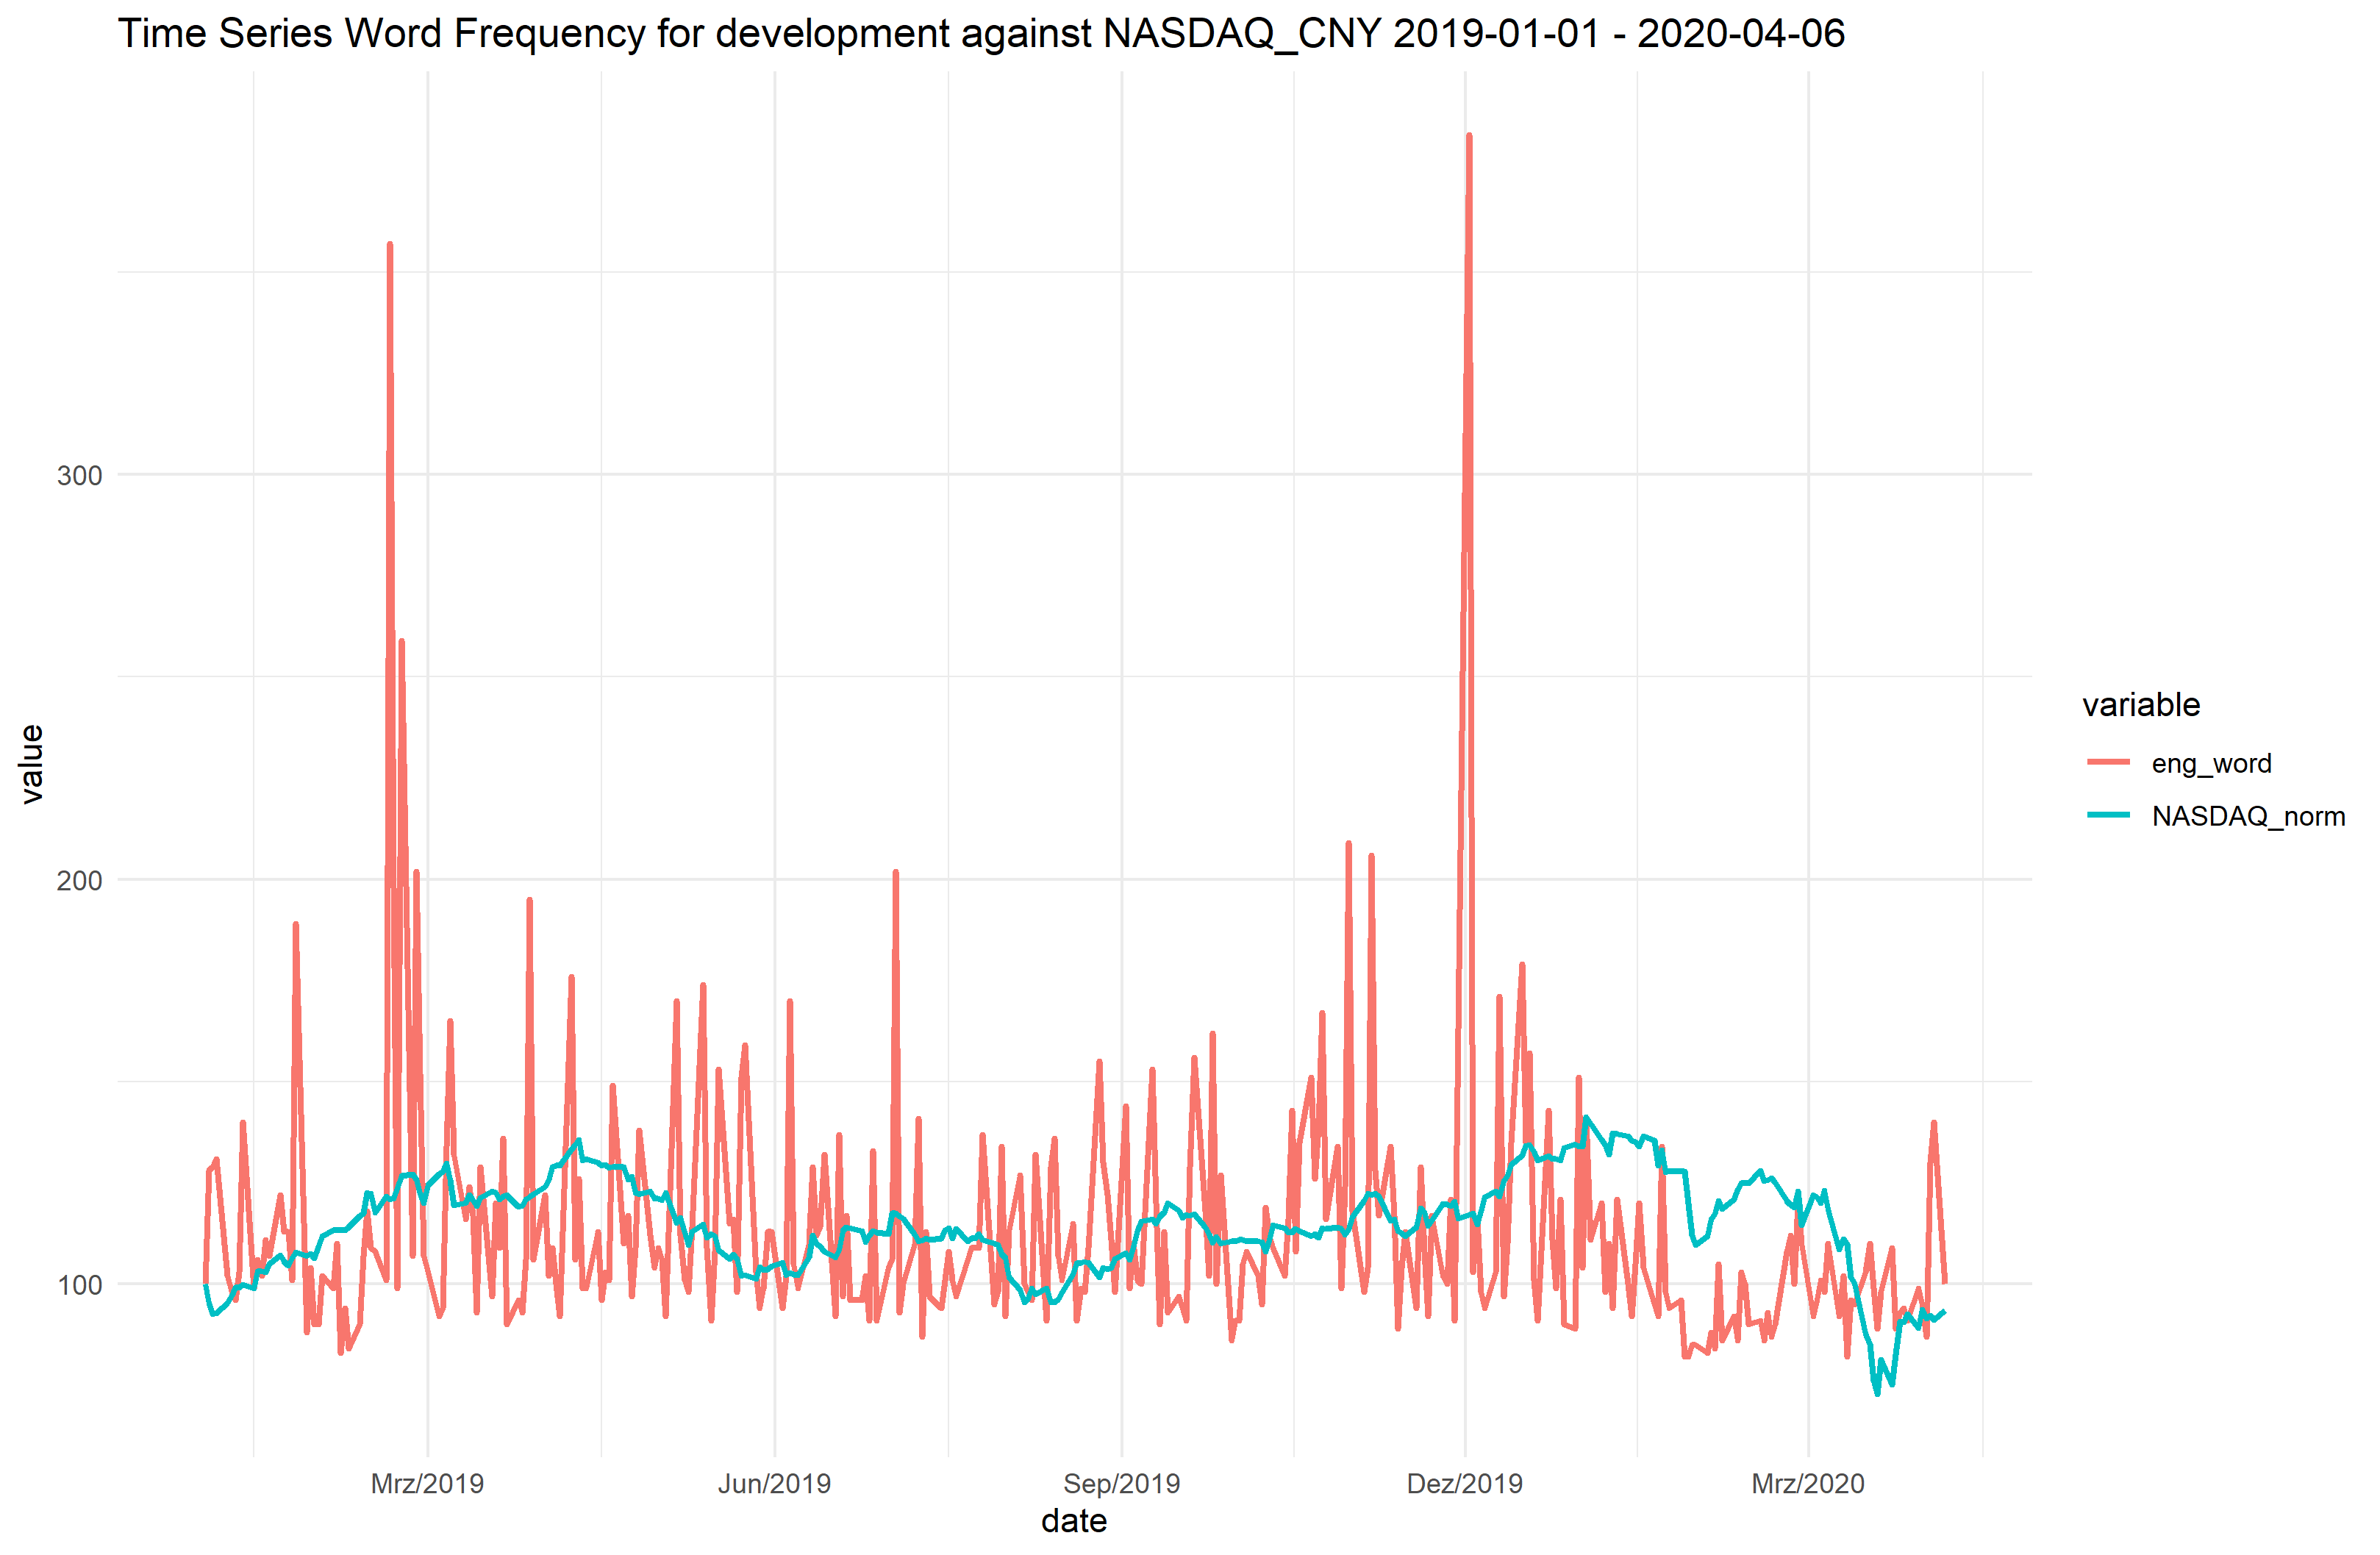
\includegraphics[width=0.49\linewidth,height=0.2\textheight]{C:/Users/David/Seafile/Meine Bibliothek/Kurse/adv-r/Advanced_R_Project/ts_plots/development} 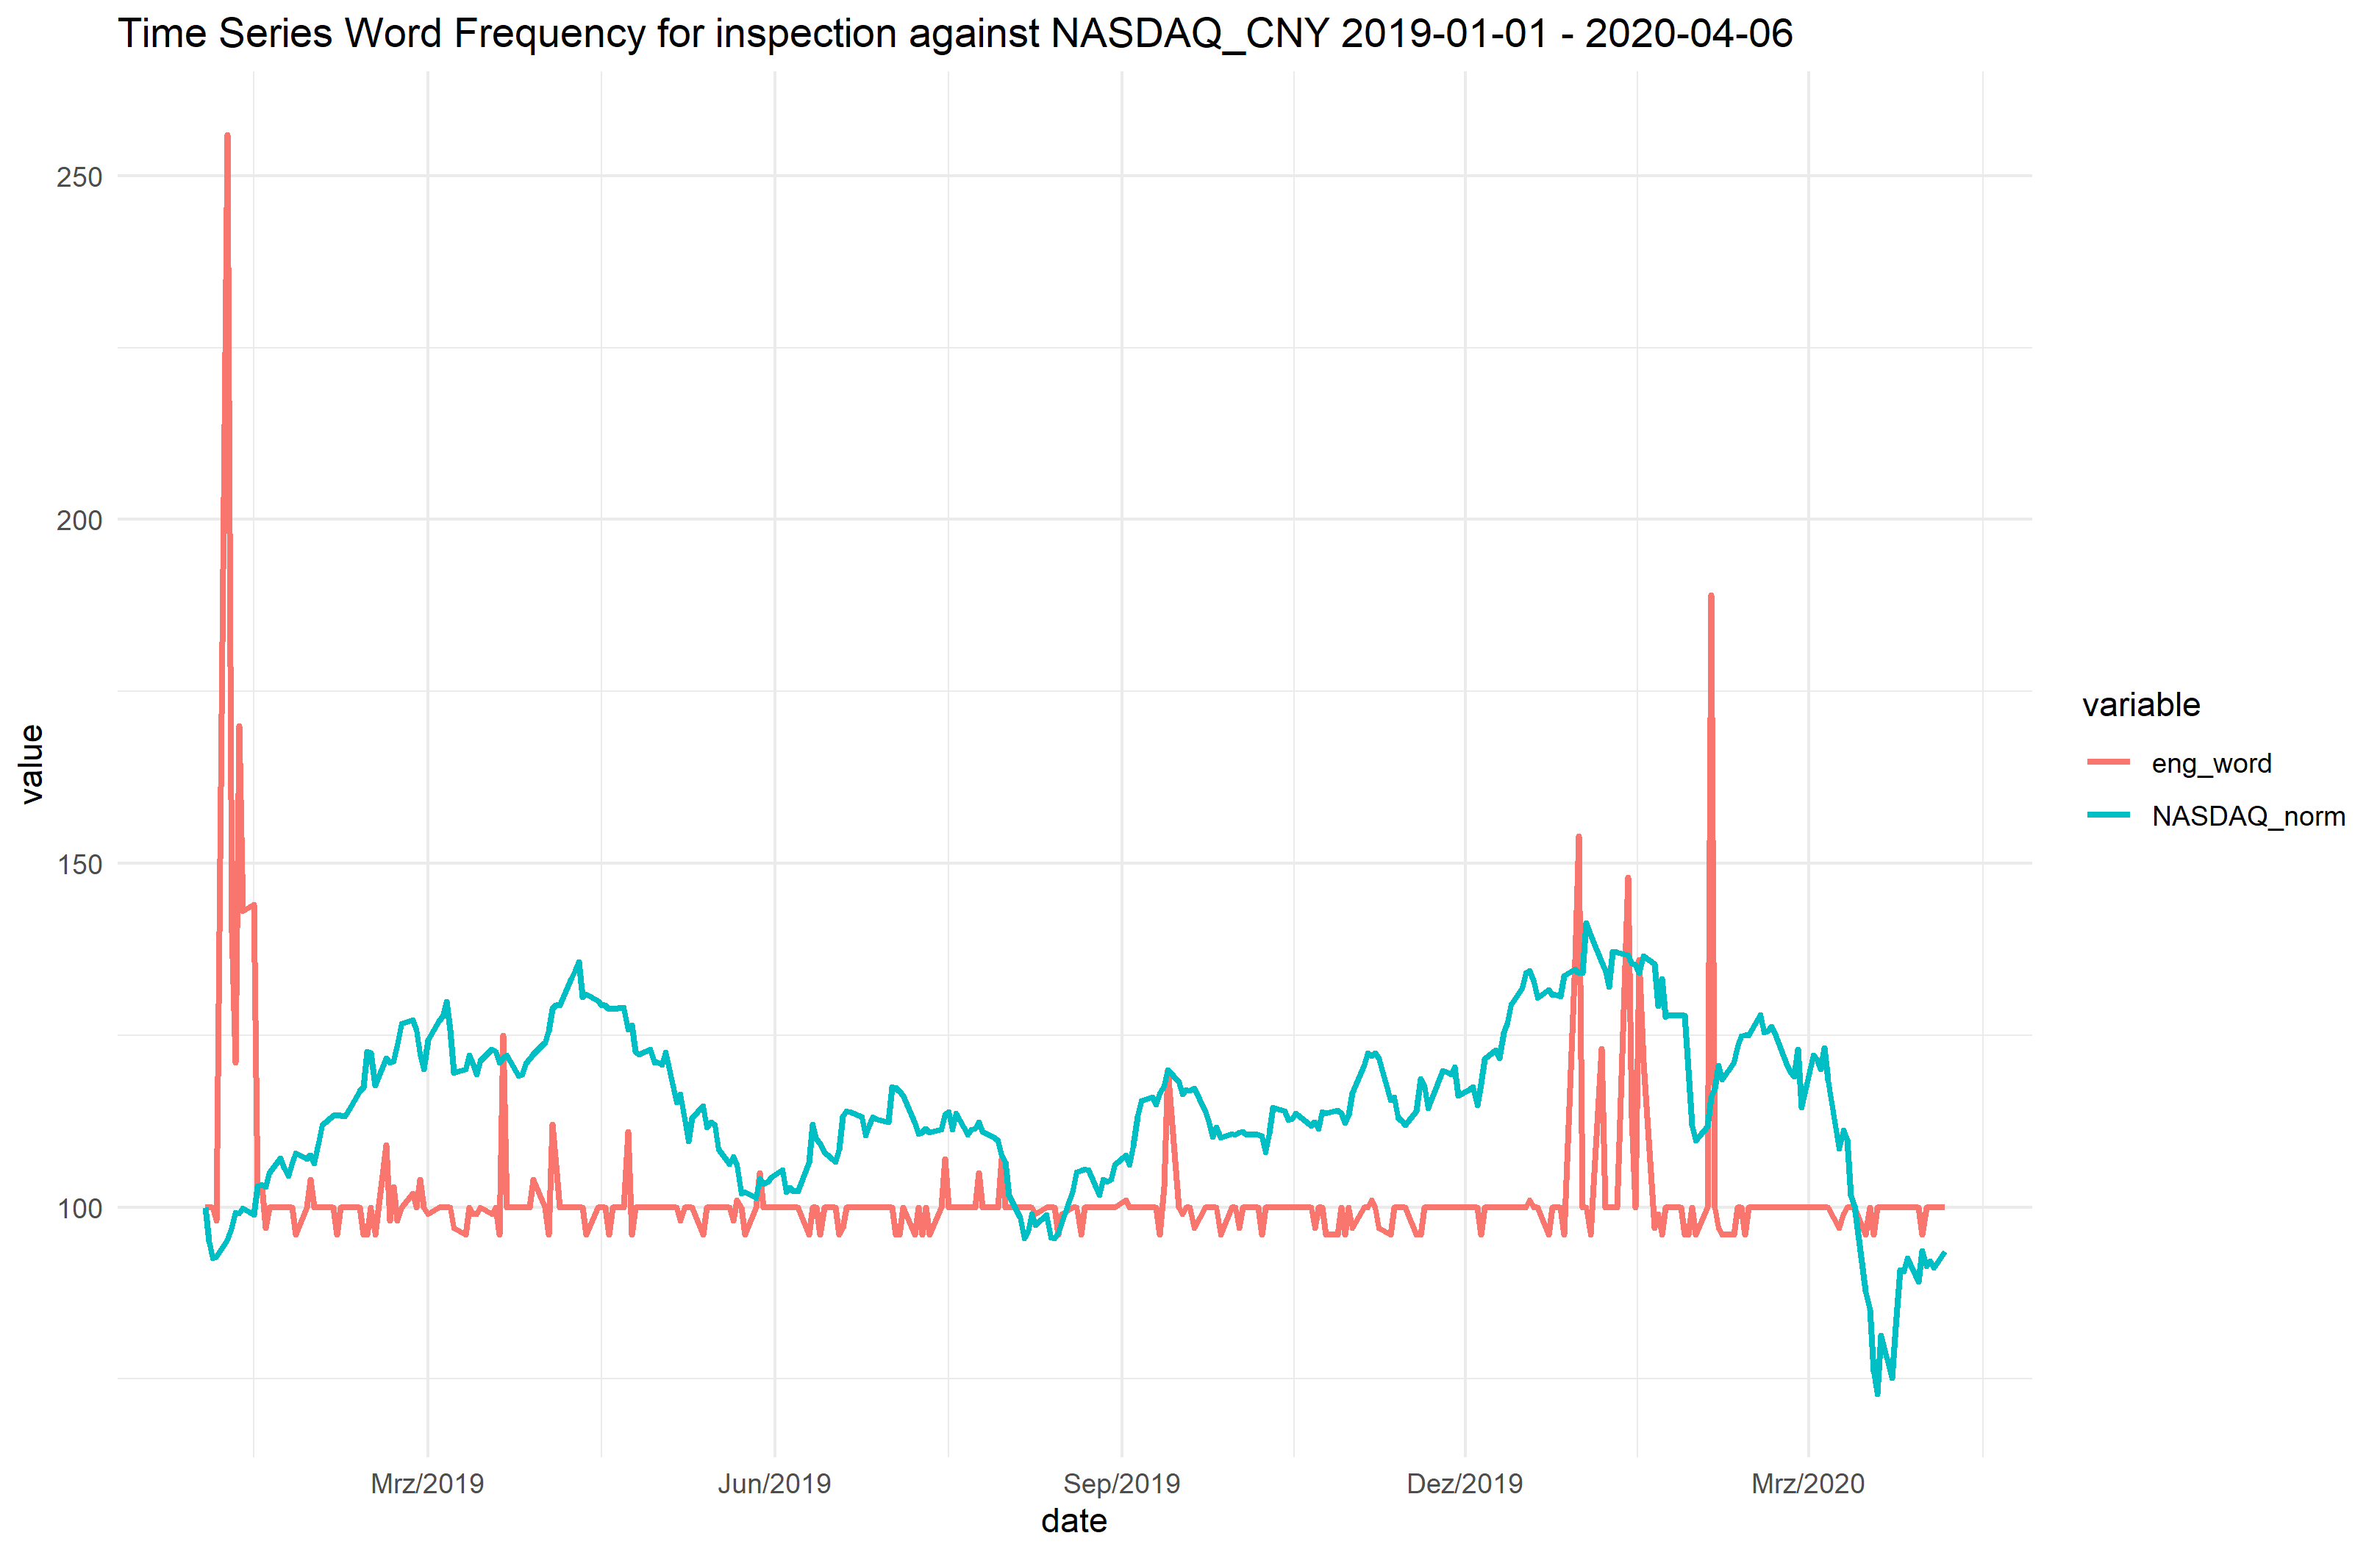
\includegraphics[width=0.49\linewidth,height=0.2\textheight]{C:/Users/David/Seafile/Meine Bibliothek/Kurse/adv-r/Advanced_R_Project/ts_plots/inspection} 

}

\end{figure}

\hypertarget{interesting-extensions}{%
\subsubsection{Interesting extensions}\label{interesting-extensions}}

More classical text analysis output would have to include of course the
most common words per article. This is a straighforward way of gaining a
better understanding of a corpus. Even more interesting is comparing
different parts of the same corpus, e.g.~at different time points. This
would show systematic deviations in use of vocabulary, e.g.~before and
after the crisis.

Correlations are another way to reveal underlying structures of the
text. Which two- or n-word groups are particularly common? How does
their use vary over time? R packages including plots for these so-called
\enquote{n-grams} include the aptly named
\enquote{ngram},\enquote{JSTORr}, \enquote{NSP} and \enquote{WordStat}.

\hypertarget{advanced-options}{%
\subsubsection{Advanced options}\label{advanced-options}}

On the more technical and advanced side, lda/topic models can offer
great insights, but are also more difficult to interpret. Sentiment
analysis is another complex, but controversial topic, which could be
implemented.

\hypertarget{results}{%
\section{Results}\label{results}}

Here we should show some of the results of our application. As discussed
before COVID-19 will be most likely the centre of our examples but maybe
we can show here the mentioned theory of the shadow page as well

\hypertarget{discussion}{%
\section{Discussion}\label{discussion}}

How could we improve the app? Extend the archive? Add more economic
data? Implement some other statistical information?

Encrypted server version

\hypertarget{conclusion}{%
\section{Conclusion}\label{conclusion}}

Summary of our application and our results. Do we have plans to expand
and update the app further in the near future?

Just an idea, because they want it scientific, let's include a bunch of
references to the data mining book, etc., just if you find some that
would make sense.

\newpage
\renewcommand*{\mkbibnamefamily}[1]{\textbf{#1}}
\renewcommand*{\mkbibnamegiven}[1]{\textbf{#1}}
\renewcommand*{\mkbibnameprefix}[1]{\textbf{#1}}
\renewcommand*{\mkbibnamesuffix}[1]{\textbf{#1}}
\printbibliography[title=References]

\newpage
\textbf{Eidesstattliche Versicherung}

\bigskip

Ich versichere an Eides statt durch meine Unterschrift, dass ich die vorstehende Arbeit selbständig und ohne fremde Hilfe angefertigt und alle Stellen, die ich wörtlich oder annähernd wörtlich aus Veröffentlichungen entnommen habe, als solche kenntlich gemacht habe, mich auch keiner anderen als der angegebenen Literatur oder sonstiger Hilfsmittel bedient habe. Die Arbeit hat in dieser oder ähnlicher Form noch keiner anderen Prüfungsbehörde vorgelegen.

\vspace{1cm}
\rule{0pt}{2\baselineskip} %
\par\noindent\makebox[2.25in]{\indent Essen, den \hrulefill} \hfill\makebox[2.25in]{\hrulefill}%
\par\noindent\makebox[2.25in][l]{} \hfill\makebox[2.25in][c]{David Schulze, Eyayaw Teka Beze, Paffen}%


\end{document}
